\documentclass[slidestop,compress,xcolor=table,mathserif,hyperref={bookmarks=false}]{beamer}
\usetheme{TACC}

\usepackage{tikz}
\usetikzlibrary{automata,shapes,arrows}
\usepackage{lmodern}
\usepackage[overlay]{textpos}
\usepackage[applemac]{inputenc}
\usepackage{pgfpages}
\usepackage{multirow}

\newenvironment<>{varblock}[2][.9\textwidth]{%
  \setlength{\textwidth}{#1}
  \begin{actionenv}#3%
    \def\insertblocktitle{#2}%
    \par%
    \usebeamertemplate{block begin}}
  {\par%
    \usebeamertemplate{block end}%
  \end{actionenv}}

\author{\textbf{\Large{Leo Fialho, Ashay Rane and Jim Browne}}}
\begin{document}

\AtBeginSection[]{
	\frame<beamer>{
		\frametitle{Agenda}
		\begin{columns}[c]
			\begin{column}{0.5\textwidth}
				\tableofcontents[currentsection,subsectionstyle=shadow/hide/hide]
			\end{column}
			\begin{column}{0.5\textwidth}
				\pgfuseimage{configuration}
			\end{column}
		\end{columns}
	}
}

%------------------------------------------------------------
\pgfdeclareimage[interpolate=true,width=5cm]{logo_TACC}{figures/tacc}
\pgfdeclareimage[interpolate=true,width=5cm]{logo_UT}{figures/ut}
\pgfdeclareimage[interpolate=true,width=1.5cm]{logo_TACC_small}{figures/tacc}
\pgfdeclareimage[interpolate=true,width=1cm]{logo_UT_small}{figures/ut}
\pgfdeclareimage[interpolate=true,width=6cm]{configuration}{figures/configuration}

%------------------------------------------------------------
\title{\textbf{\Huge Automatic\\ Performance Optimization\\with PerfExpert\\}}
\date{\pgfuseimage{logo_TACC} \ \ \pgfuseimage{logo_UT}}
\logo{\pgfuseimage{logo_TACC_small} \ \ \ \pgfuseimage{logo_UT_small}}
\frame[plain]{\titlepage}

%------------------------------------------------------------
\section{Introduction}
\subsection{Introduction}
\frame{\frametitle{Introduction} \pause
	\begin{exampleblock}{Steps for Performance Optimization} \pause
		\begin{itemize}
			\item Metrics definition and performance measurement \\[2mm] \pause
			\item Analysis, diagnosis and identification of bottlenecks \\[2mm] \pause
			\item Recommendation of optimizations \\[2mm] \pause
			\item Implementation of the recommended optimizations \\[2mm] \pause
		\end{itemize}
	\end{exampleblock}

	\begin{block}{Challenges of Automatic Performance Optimization} \pause
		\begin{itemize}
			\item Programmers are really inventive \\[2mm] \pause
			\item The execution environment is quite complex \\[2mm] \pause
			\item Compilers usually do only static source code analysis \\[2mm]
		\end{itemize}
	\end{block}
}

%------------------------------------------------------------
\section{The New PerfExpert}
\subsection{The New PerfExpert}
\frame{\frametitle{Current Version: The Big Picture}
	\begin{picture}(0,0)(0,0)
		\put(-28,-160){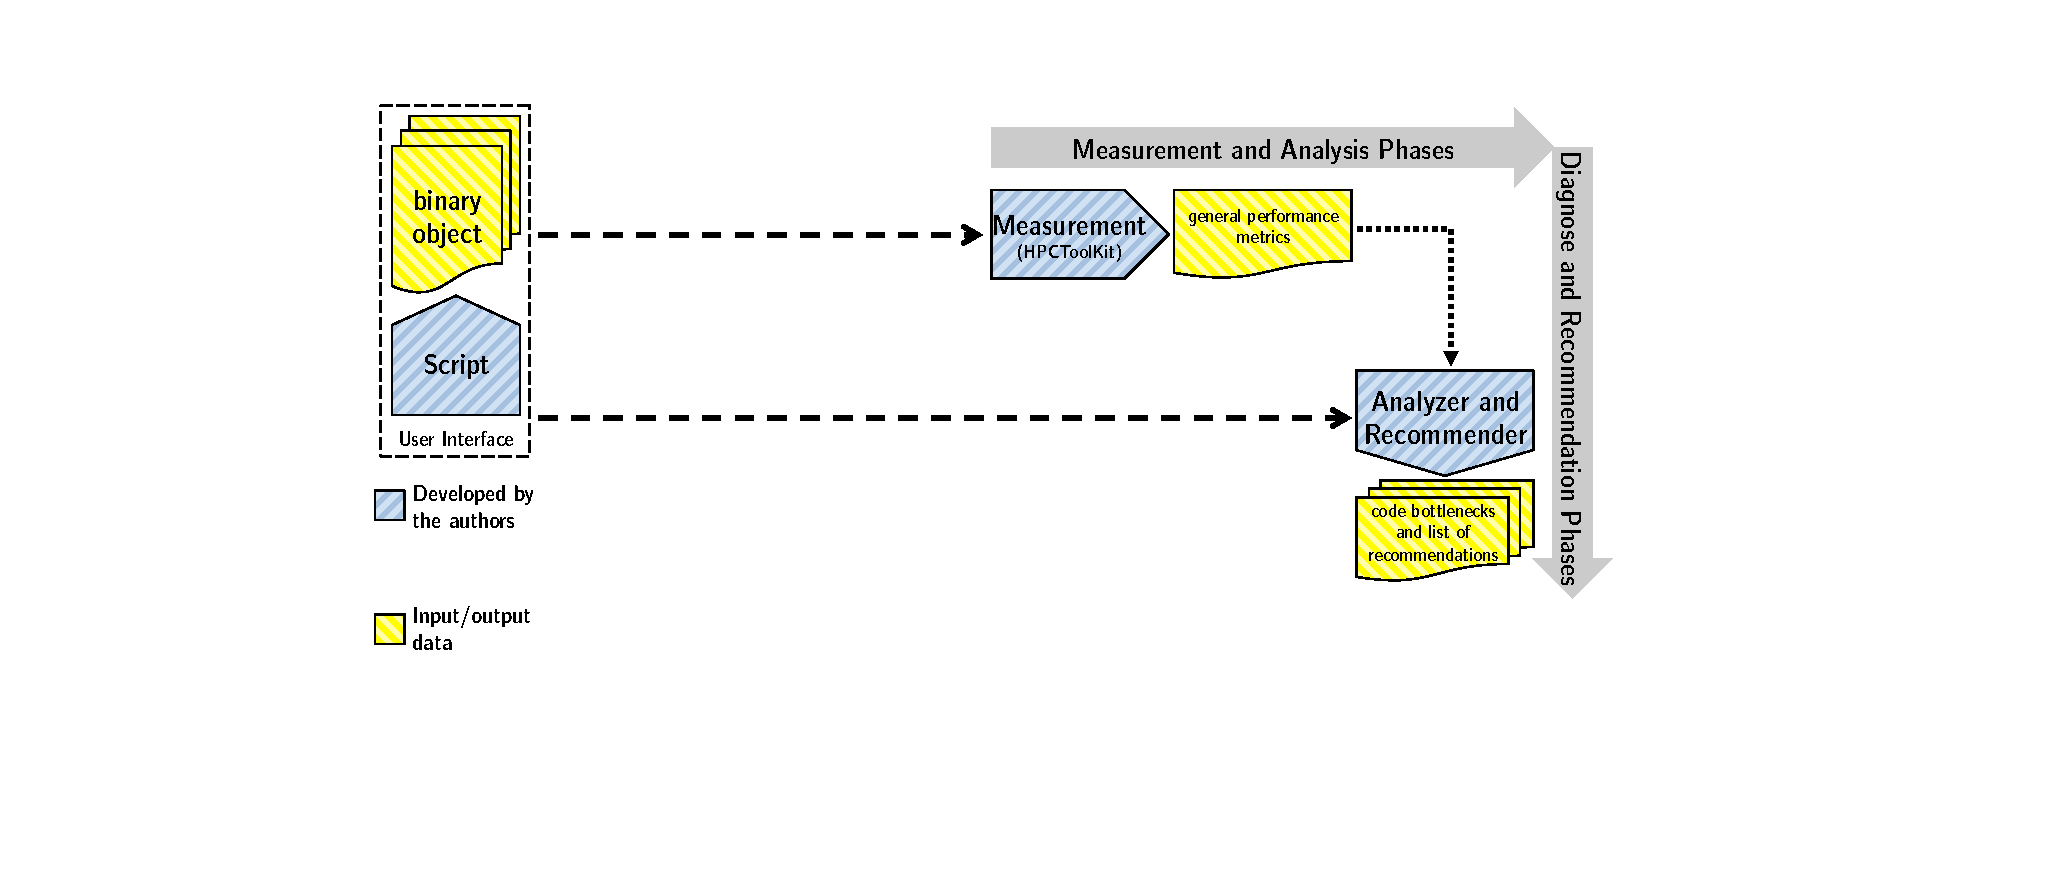
\includegraphics[width=12.8cm]{figures/pe_before}}
	\end{picture}
}

\frame{\frametitle{New Version: The Big Picture}
	\begin{picture}(0,0)(0,0)
		\put(-28,-160){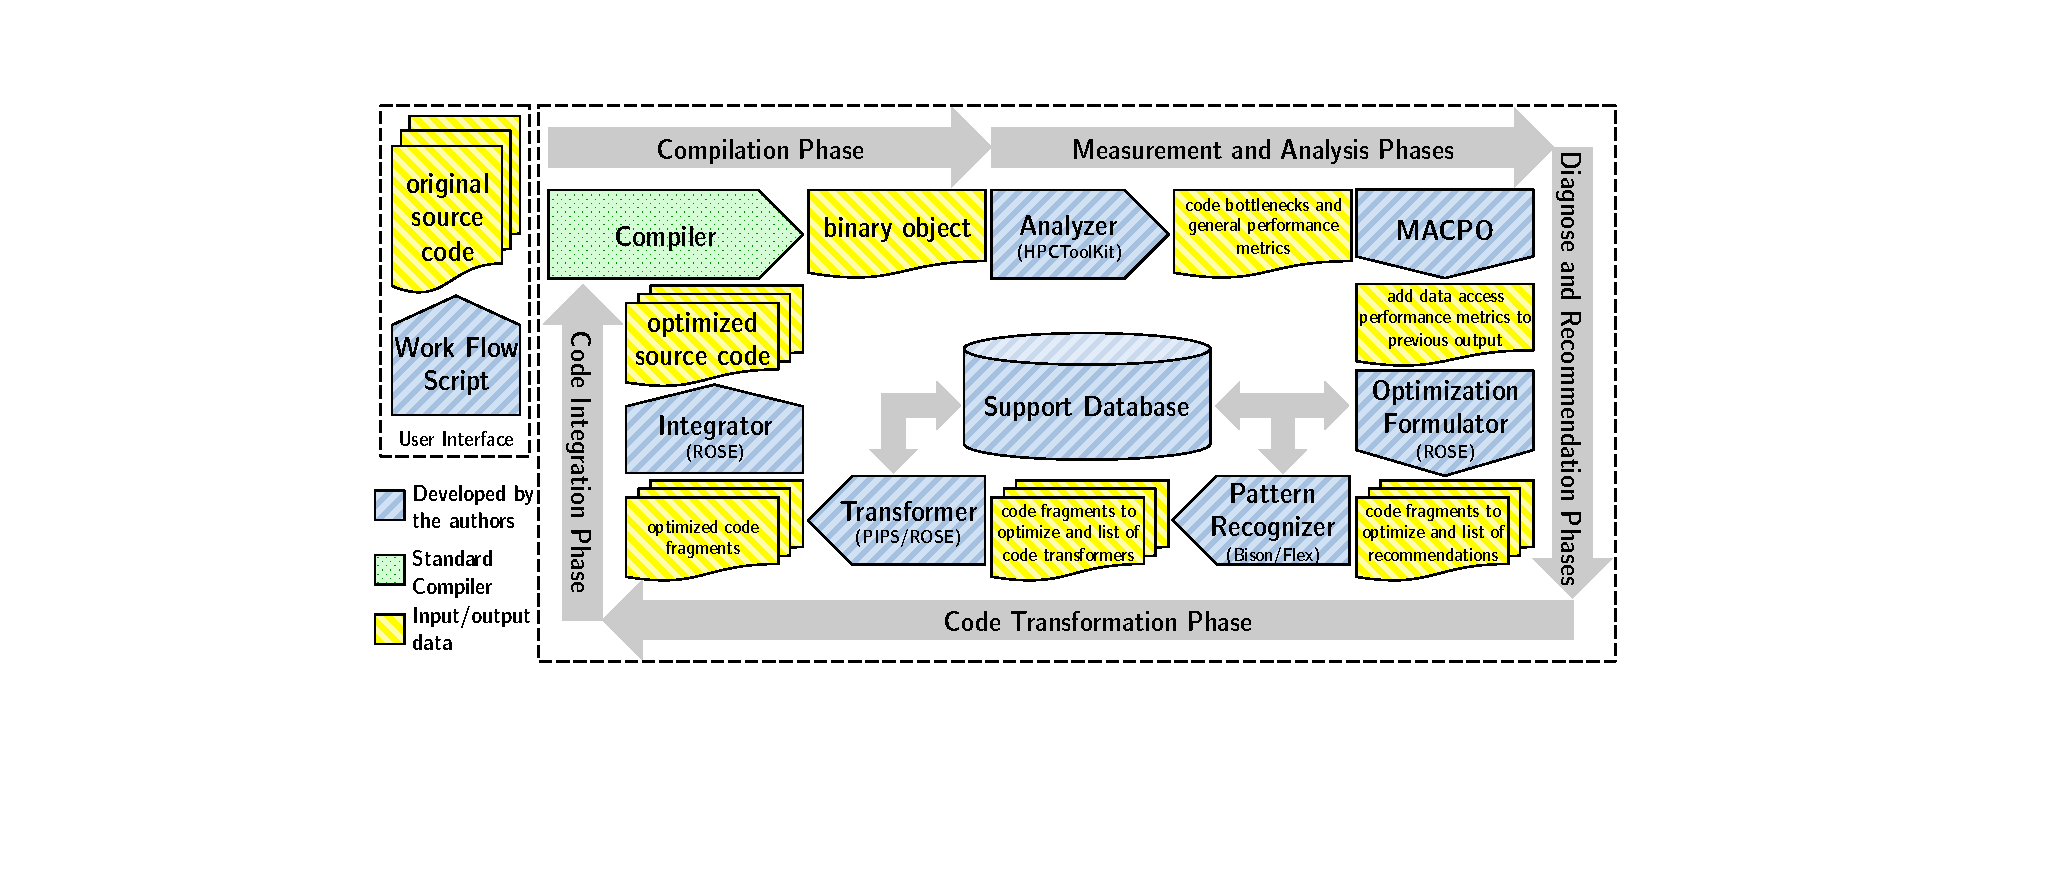
\includegraphics[width=12.8cm]{figures/pe_after}}
	\end{picture}
}

\frame{\frametitle{New Version: Short Demo}
	\vspace{2.5cm}
	\begin{center}
		\textit{\textbf{\Huge{Short demo}}}
	\end{center}
}

\frame{\frametitle{New Version: Work Flow Script}
	\begin{picture}(0,0)(0,0)
		\put(-28,-160){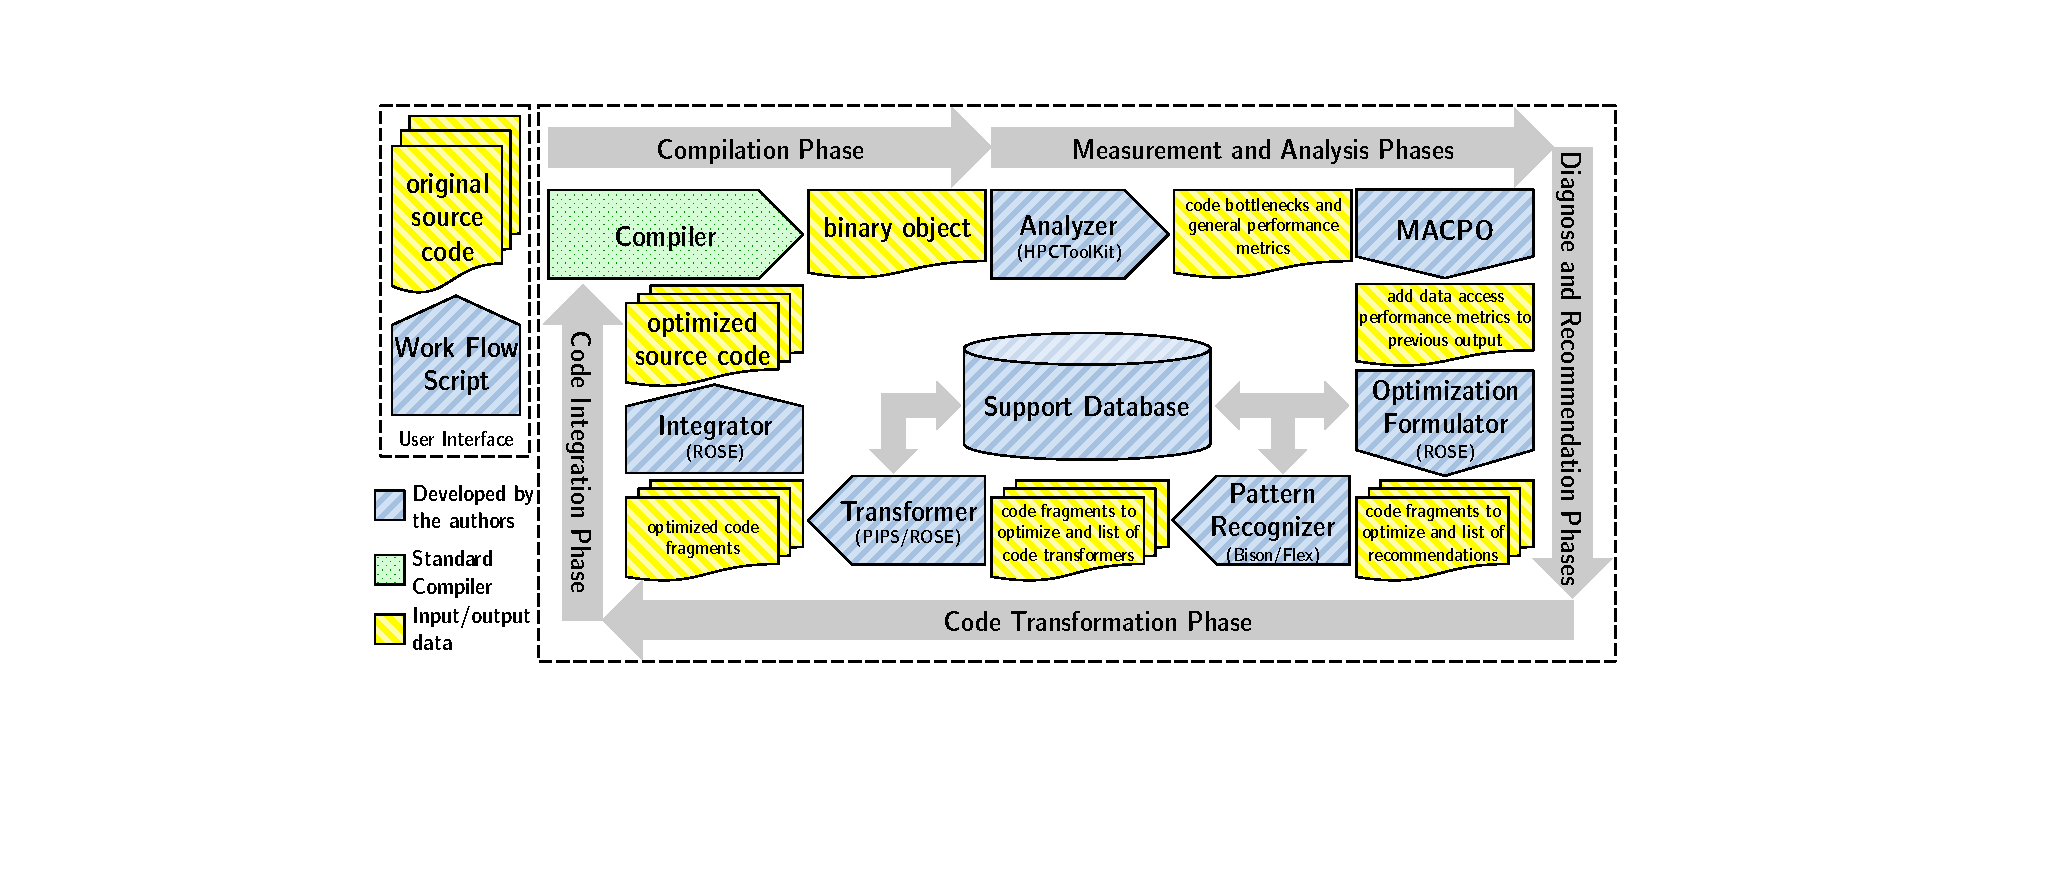
\includegraphics[width=12.8cm]{figures/pe_after}}
	\end{picture} \pause
	\begin{columns}[c]
		\begin{column}{0.09\textwidth}
		\end{column}
		\begin{column}{0.43\textwidth}
			\vspace{1.5cm}
			\begin{block}{}
				\begin{itemize}
					\item This is a shell script \\[2mm] \pause
					\item Accepts parameters \\[2mm] \pause
					\item Invokes all tools (including the compiler) \\[2mm] \pause
					\item Backward compatible \\[2mm]
				\end{itemize}
			\end{block}
		\end{column}
		\begin{column}{0.48\textwidth}
		\end{column}
	\end{columns}
}

\frame{\frametitle{New Version: Analyzer}
	\begin{picture}(0,0)(0,0)
		\put(-28,-160){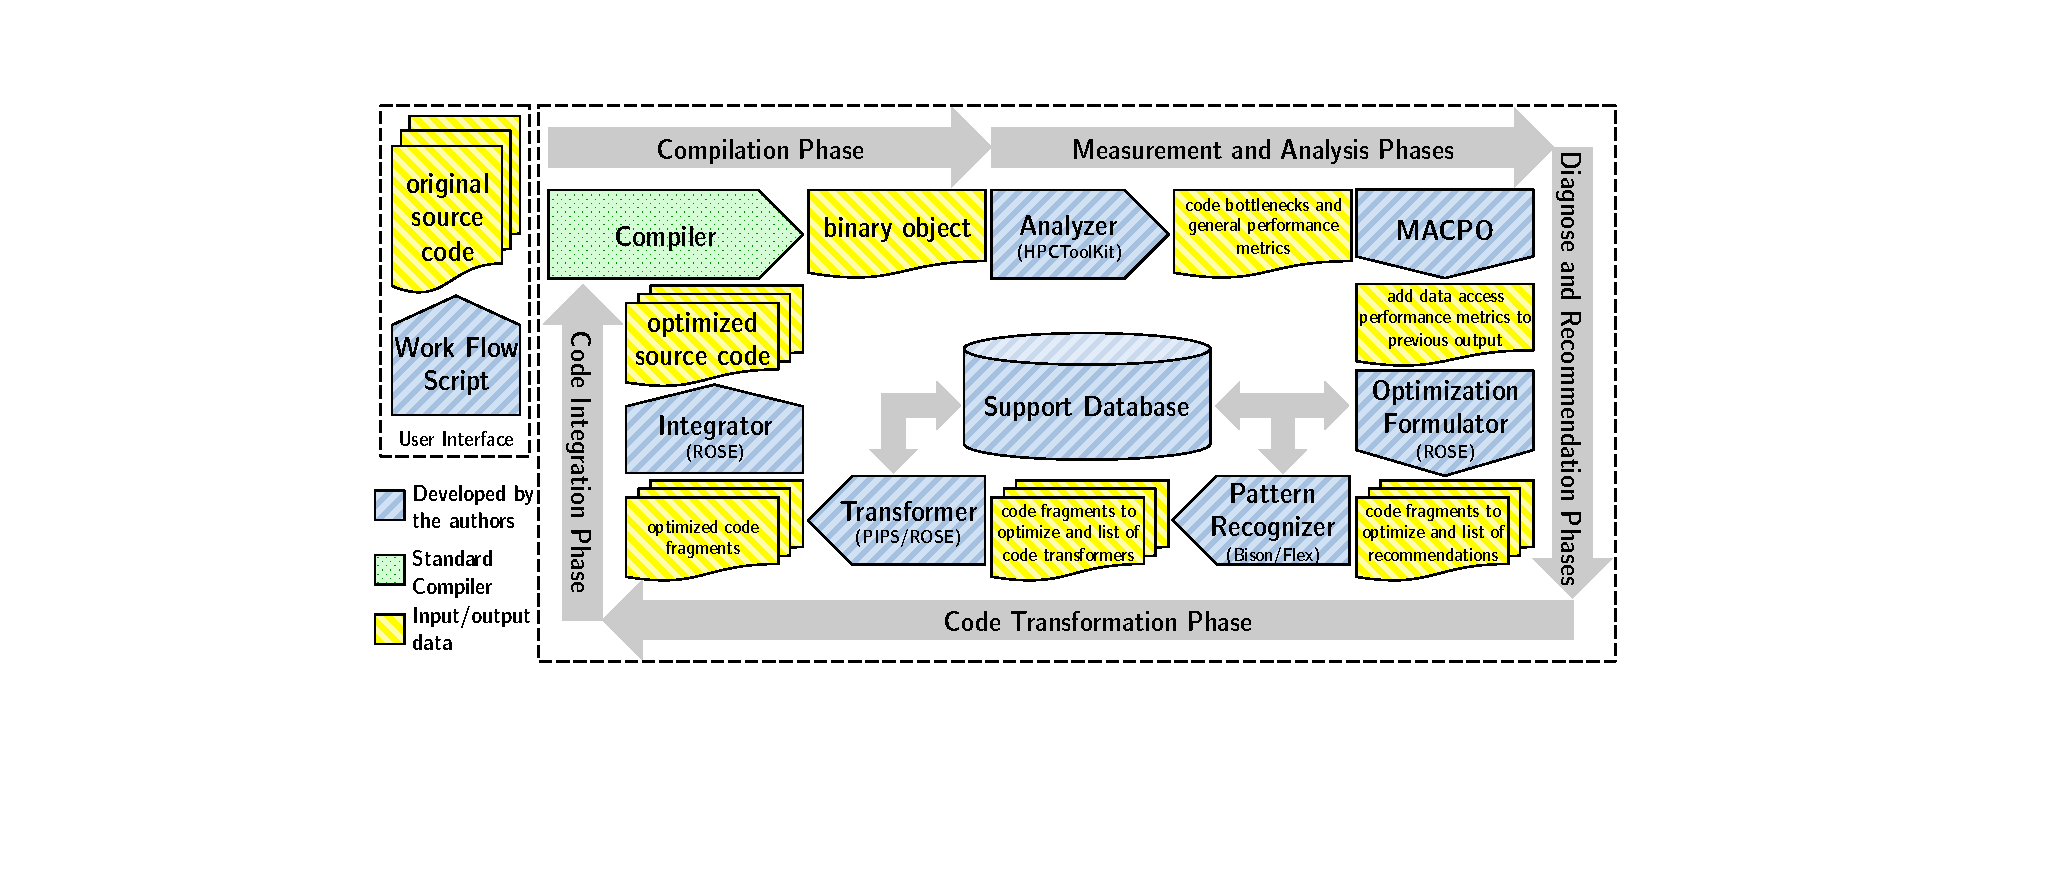
\includegraphics[width=12.8cm]{figures/pe_after}}
	\end{picture} \pause
	\begin{columns}[c]
		\begin{column}{0.35\textwidth}
		\end{column}
		\begin{column}{0.46\textwidth}
			\vspace{1.5cm}
			\begin{block}{}
				\begin{itemize}
					\item This is the old PerfExpert, minus ``recommender'' \\[2mm] \pause
					\item Based on HPCToolKit \\[2mm]
				\end{itemize}
			\end{block}
		\end{column}
		\begin{column}{0.19\textwidth}
		\end{column}
	\end{columns}
}

\frame{\frametitle{New Version: MACPO}
	\begin{picture}(0,0)(0,0)
		\put(-28,-160){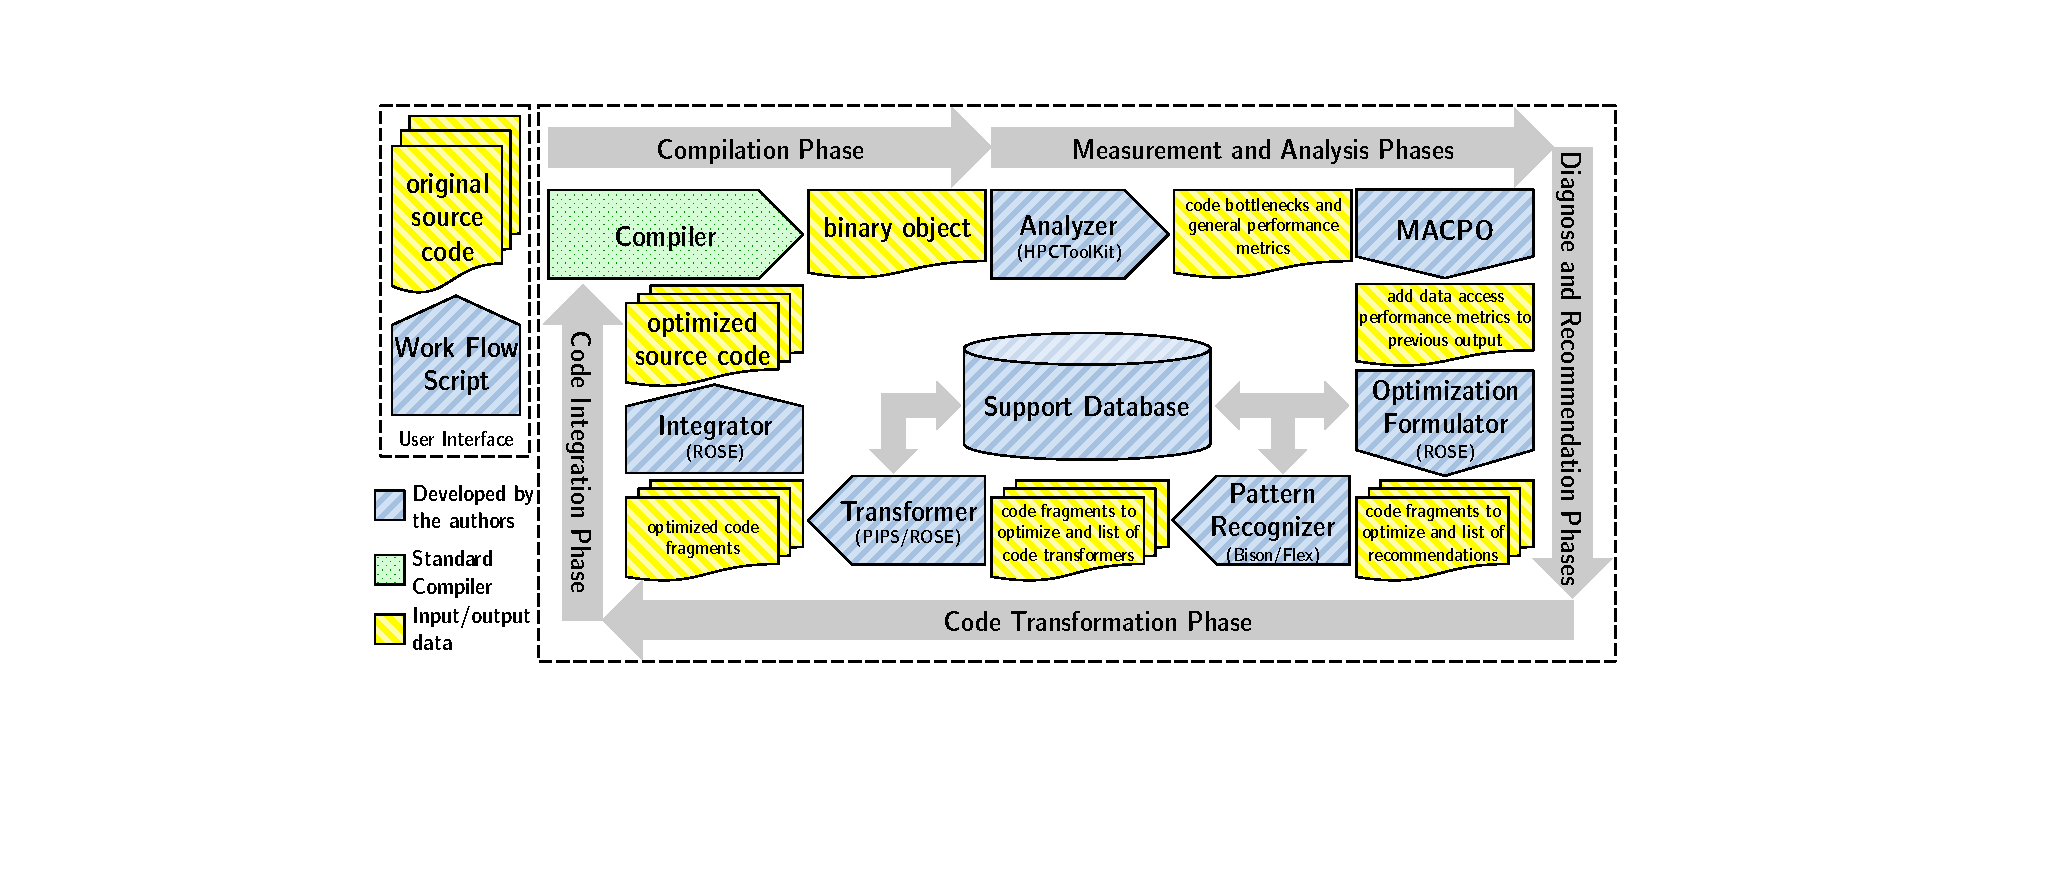
\includegraphics[width=12.8cm]{figures/pe_after}}
	\end{picture} \pause
	\begin{columns}[c]
		\begin{column}{0.35\textwidth}
		\end{column}
		\begin{column}{0.46\textwidth}
			\vspace{1.5cm}
			\begin{block}{}
				\begin{itemize}
					\item Enhances the set of metrics with data access performance metrics \\[2mm] \pause
					\item Based on ROSE \\[2mm]
				\end{itemize}
			\end{block}
		\end{column}
		\begin{column}{0.19\textwidth}
		\end{column}
	\end{columns}
}

\frame{\frametitle{New Version: Optimization Formulator}
	\begin{picture}(0,0)(0,0)
		\put(-28,-160){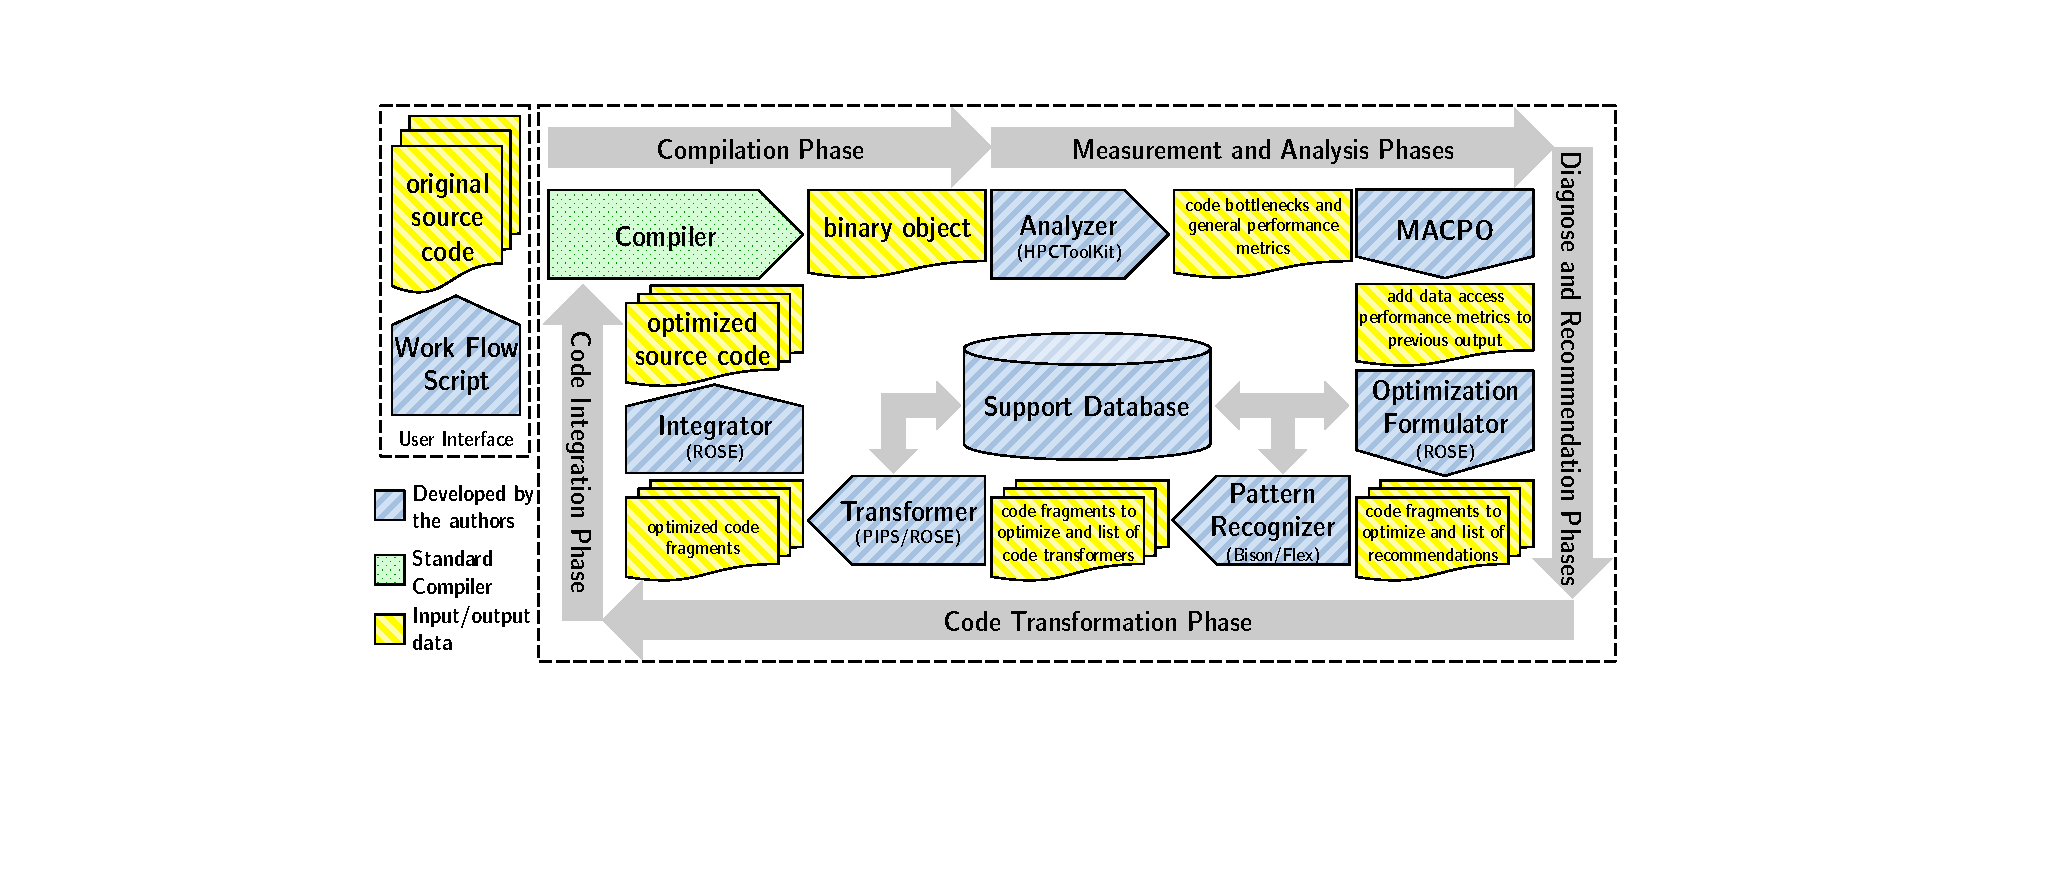
\includegraphics[width=12.8cm]{figures/pe_after}}
	\end{picture} \pause
	\begin{columns}[c]
		\begin{column}{0.86\textwidth}
			\begin{block}{}
				\begin{itemize}
					\item Loads performance metrics on the Support Database \\[2mm] \pause
					\item Runs all \textit{``recommendation selection functions''} \\[2mm] \pause
					\item Concatenates and ranks the list of recommendations \\[2mm] \pause
					\item Extracts code fragments identified as bottlenecks \\[2mm] \pause
					\item Based on ROSE \\[2mm] \pause
					\item \textbf{Extendable:} accepts user-defined performance metrics \\[2mm] \pause
					\item \textbf{Extendable:} it is possible to write new \textit{``recommendation selection functions''} (SQL query) \\[2mm]
				\end{itemize}
			\end{block}
		\end{column}
		\begin{column}{0.19\textwidth}
		\end{column}
	\end{columns}
}

\frame{\frametitle{New Version: Support Database}
	\begin{picture}(0,0)(0,0)
		\put(-28,-160){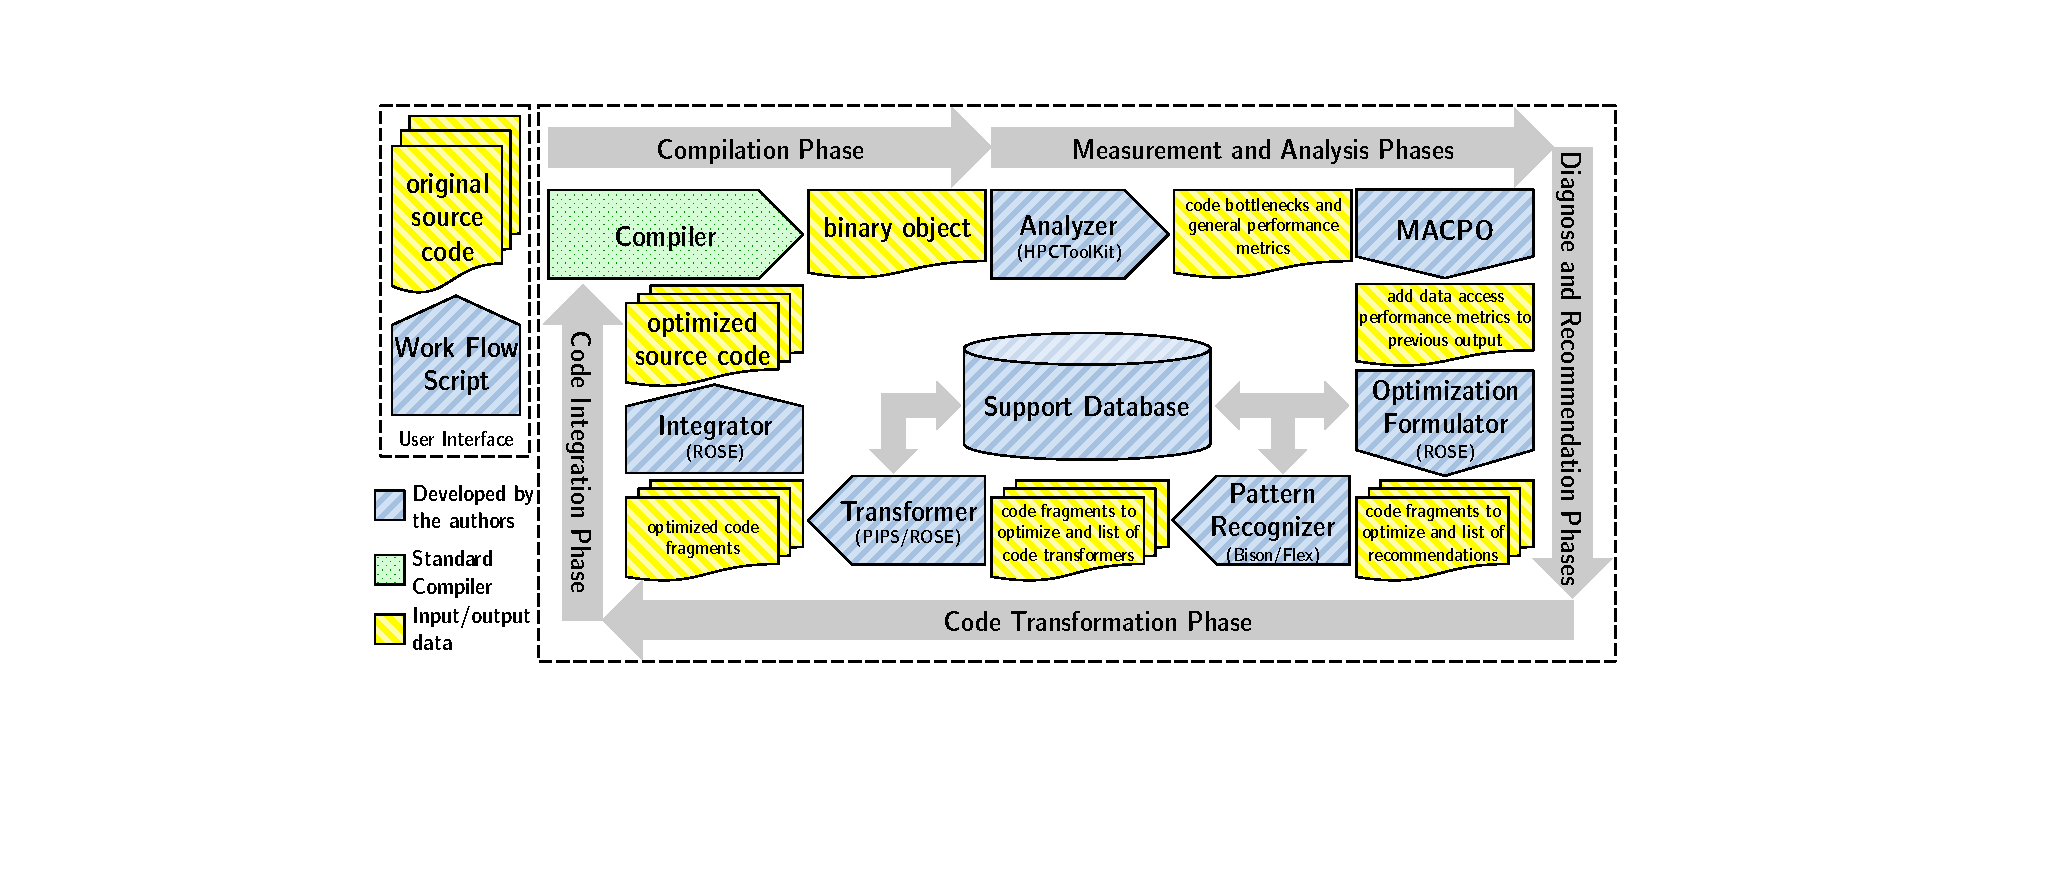
\includegraphics[width=12.8cm]{figures/pe_after}}
	\end{picture} \pause
	\begin{columns}[c]
		\begin{column}{0.1\textwidth}
		\end{column}
		\begin{column}{0.96\textwidth}
			\vspace{-0.8cm}
			\begin{block}{}
				\begin{itemize}
					\item This is a SQLite database \\[2mm] \pause
					\item Stores the list of \textit{``recommendation selection functions''}, \textit{``pattern recognizers''} and \textit{``code transformers''} \\[2mm] \pause
					\item Engine to run the \textit{``recommendation selection functions''}
				\end{itemize}
			\end{block}
		\end{column}
	\end{columns}
}

\frame{\frametitle{New Version: Pattern Recognizer}
	\begin{picture}(0,0)(0,0)
		\put(-28,-160){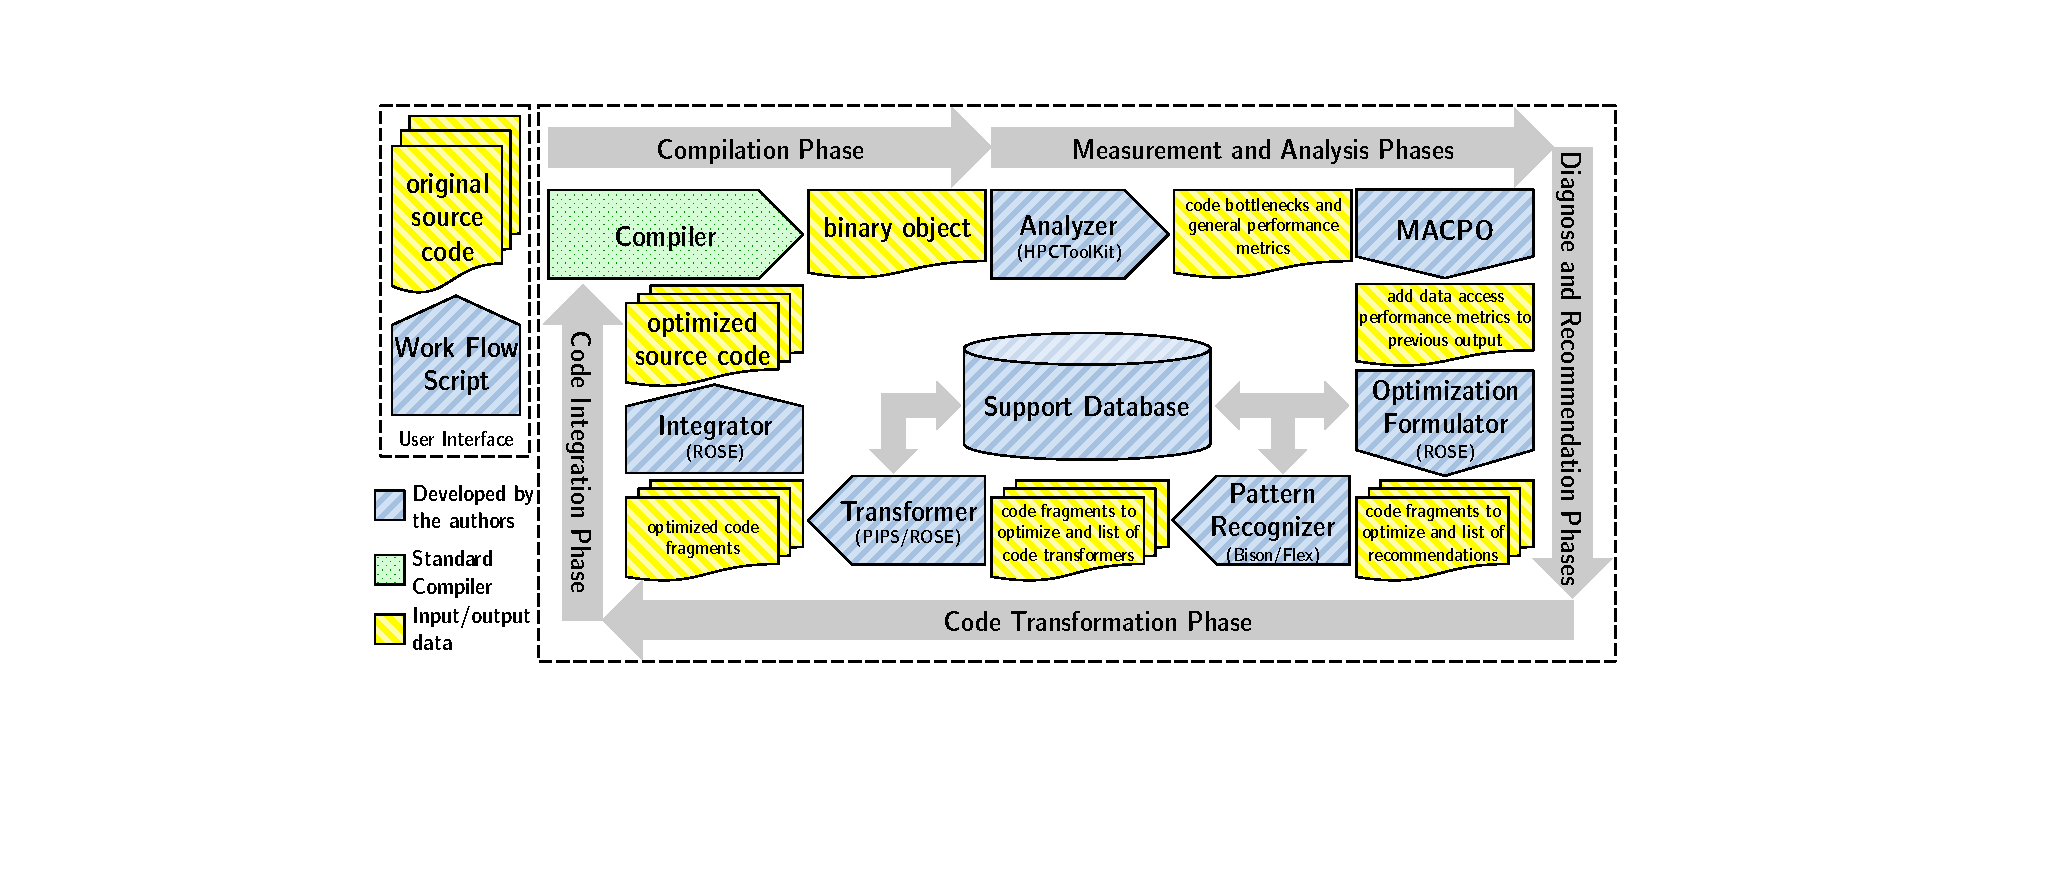
\includegraphics[width=12.8cm]{figures/pe_after}}
	\end{picture} \pause
	\begin{columns}[c]
		\begin{column}{0.05\textwidth}
		\end{column}
		\begin{column}{1.05\textwidth}
			\vspace{-1.2cm}
			\begin{block}{}
				\begin{itemize}
					\item Acts as a ``filter'' trying to find (match) the right code transformer for a source code fragment (identified as bottleneck) \\[2mm] \pause
					\item Language sensitive \\[2mm] \pause
					\item Based on Bison and Flex \\[2mm] \pause
					\item One recommendation may have multiple pattern recognizers \\[2mm] \pause
					\item \textbf{Extendable:} it is possible to write new grammars to recognize/ match/filter code fragments (to work with new ``transformers'') \\[2mm]
				\end{itemize}
			\end{block}
		\end{column}
	\end{columns}
}

\frame{\frametitle{New Version: Transformer}
	\begin{picture}(0,0)(0,0)
		\put(-28,-160){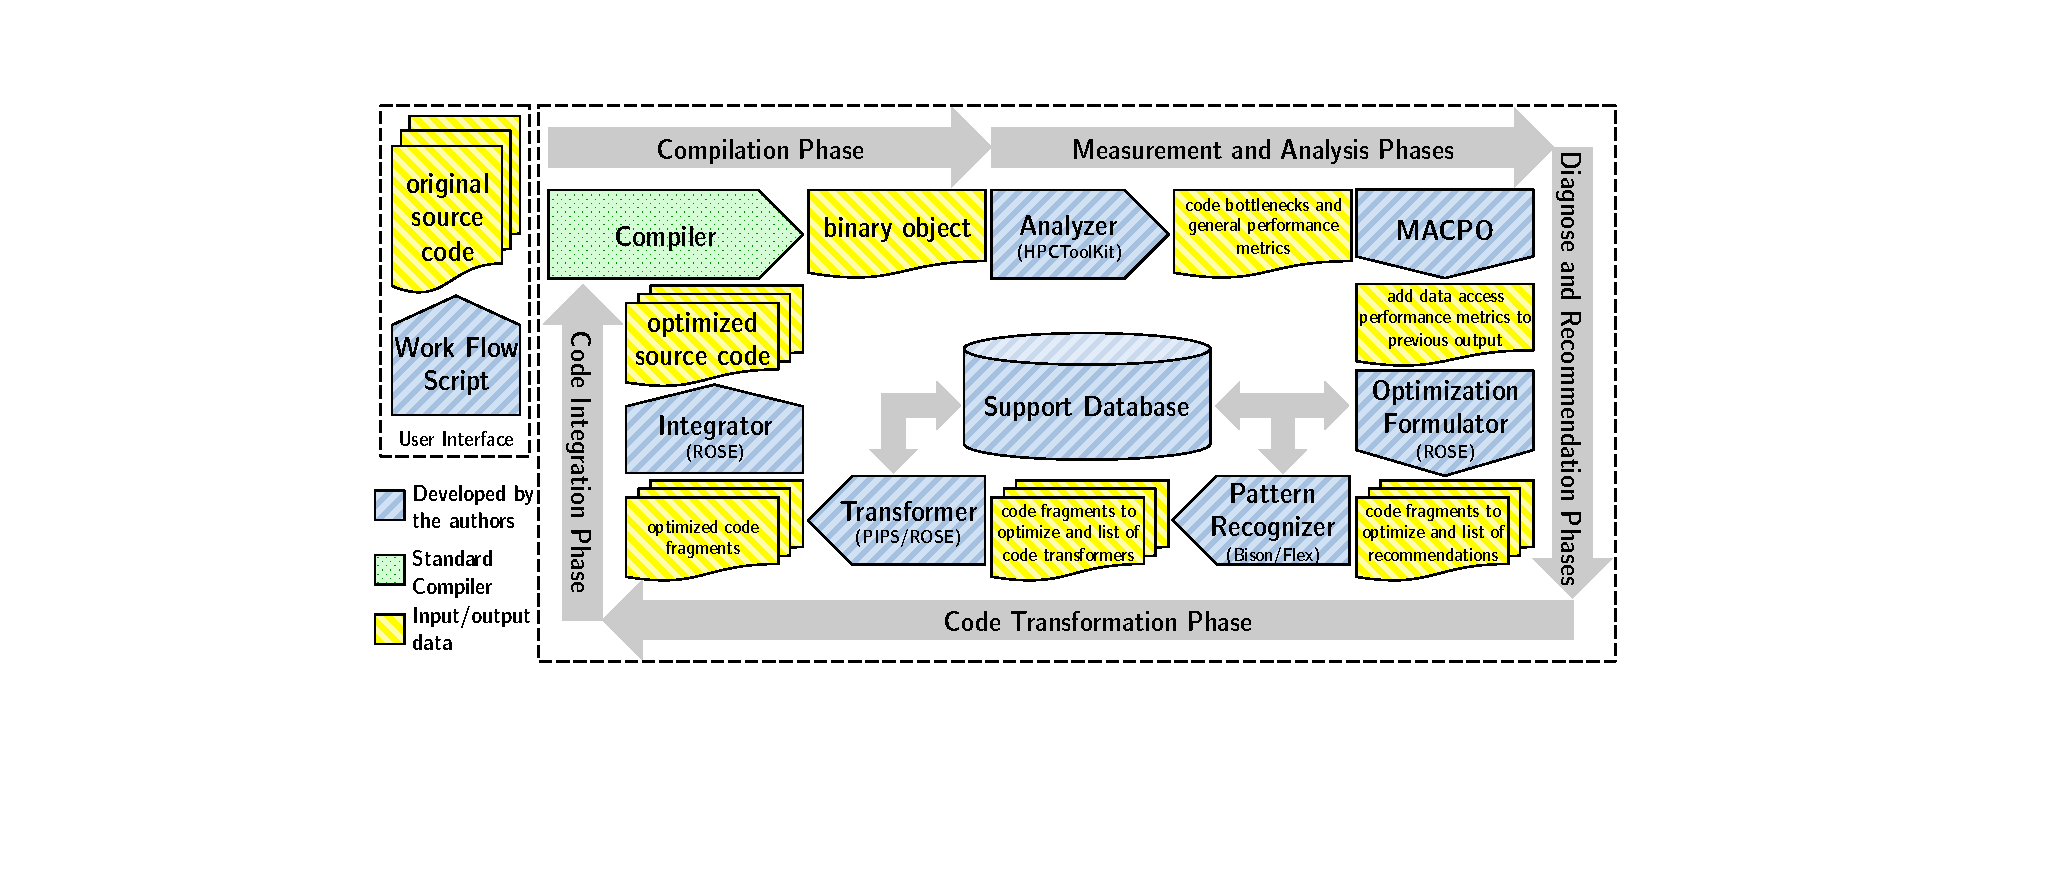
\includegraphics[width=12.8cm]{figures/pe_after}}
	\end{picture} \pause
	\vspace{-1.1cm}
	\begin{block}{}
		\begin{itemize}
			\item Implements the recommendation by applying source code transformation \\[2mm] \pause
			\item May or may not be language sensitive \\[2mm] \pause
			\item Based on ROSE, PIPS or anything you want \\[2mm] \pause
			\item One code pattern may lead to multiple code transformers \\[2mm] \pause
			\item \textbf{Extendable:} it is possible to write code transformers using any language you want \\[2mm]
		\end{itemize}
	\end{block}
}

\frame{\frametitle{New Version: Integrator}
	\begin{picture}(0,0)(0,0)
		\put(-28,-160){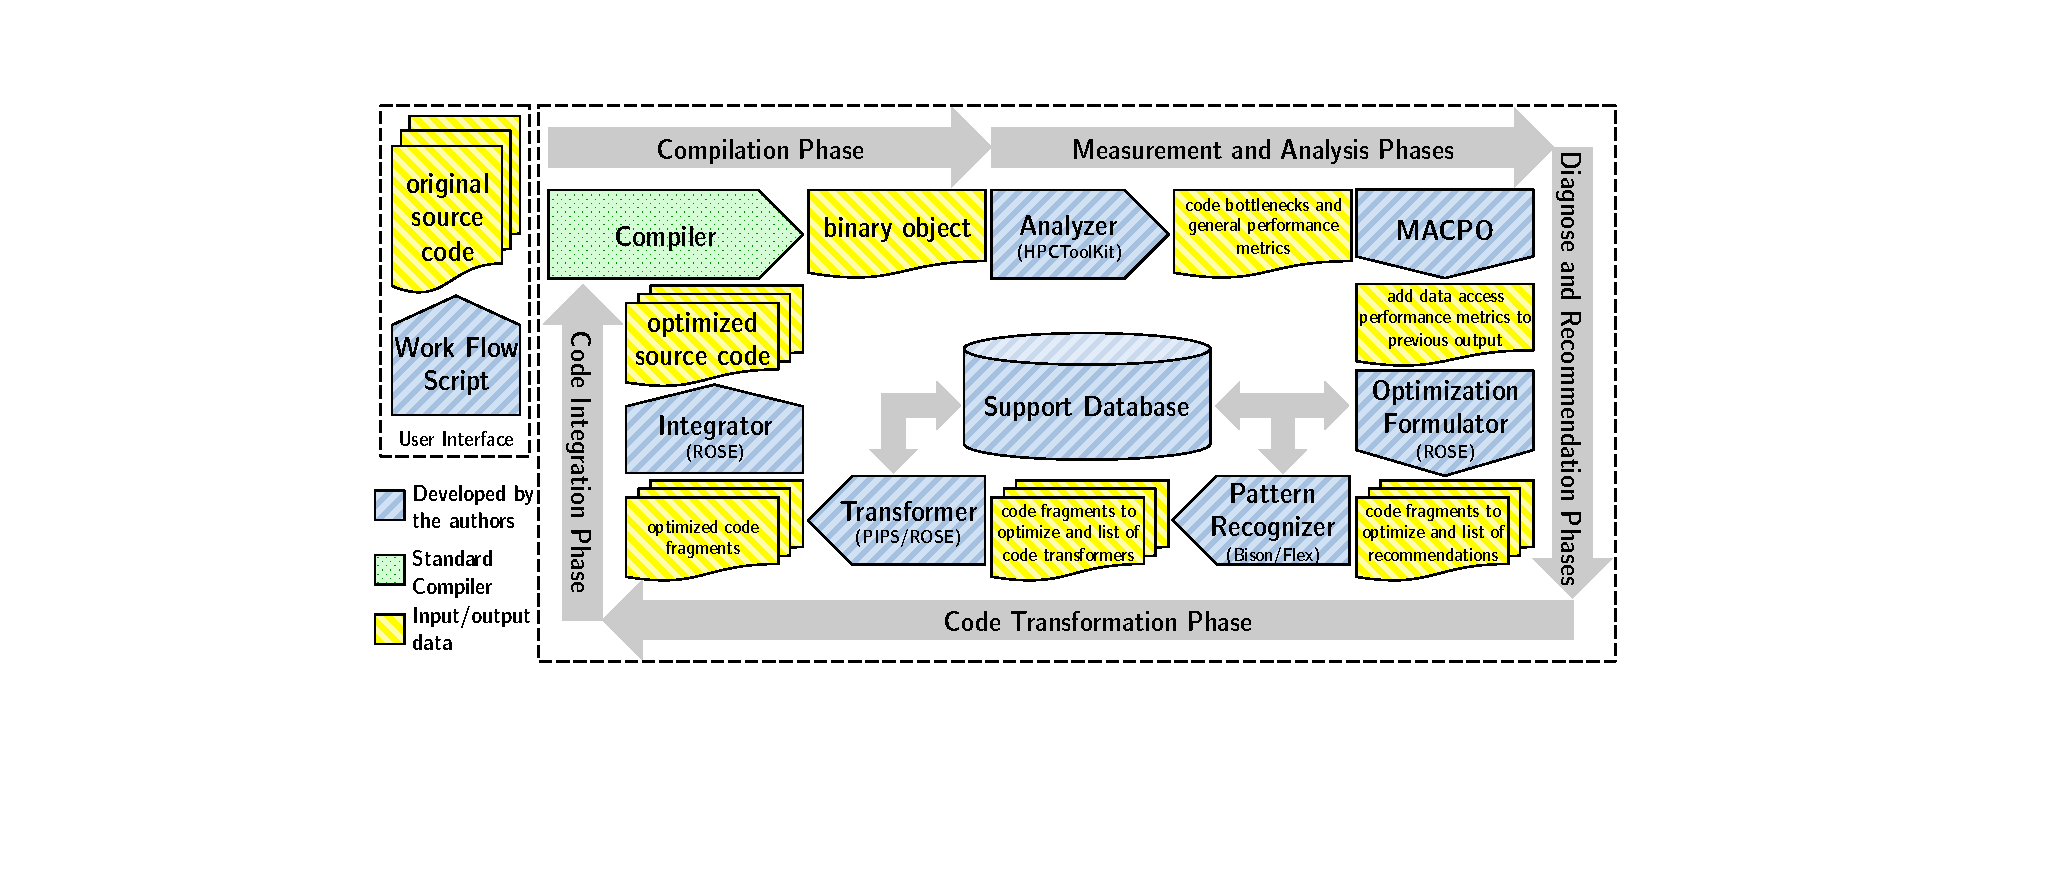
\includegraphics[width=12.8cm]{figures/pe_after}}
	\end{picture} \pause
	\begin{columns}[c]
		\begin{column}{0.35\textwidth}
		\end{column}
		\begin{column}{0.46\textwidth}
			\vspace{1.5cm}
			\begin{block}{}
				\begin{itemize}
					\item Generates a new source code by integrating to the transformed code fragments \\[2mm] \pause
					\item Based on ROSE \\[2mm]
				\end{itemize}
			\end{block}
		\end{column}
		\begin{column}{0.19\textwidth}
		\end{column}
	\end{columns}
}

\frame{\frametitle{New Version: Key Points} \pause
	\begin{block}{Why is this performance optimization ``architecture'' strong?} \pause
		\begin{itemize}
			\item Each piece of the tool chain can be updated/upgraded individually \\[2mm] \pause
			\item It is flexible: you can add new metrics as well as plug new tools to measure application performance \\[2mm] \pause
			\item It is extendable: new recommendations, transformations and strategies to select recommendations (we are counting on you!)\\[2mm] \pause
			\item Multi-language, multi-architecture, open-source and built on top of established tools \\[2mm] \pause
			\item Easy to use and lightweight!
		\end{itemize}
	\end{block}
}

%------------------------------------------------------------
\section{Conclusions}
\subsection{Conclusions}
\frame{\frametitle{Conclusions} \pause
	\begin{block}{}
		\begin{itemize}
			\item This is the first end-to-end open-source performance optimization tool (as far as we know)\\[2mm] \pause
			\item It will become more and more powerful as new recommendations, transformations and features are added \\[2mm] \pause
			\item Different from (most of) the available performance optimization tools, there is no ``big code'' (to increase in complexity until it become unusable or too hard to maintain) \\[2mm]
		\end{itemize}
	\end{block}
}

\frame{\frametitle{Next Steps} \pause
	\vspace{-0.4cm}
	\begin{block}{Major Goals}\small \pause
		\begin{itemize}
			\item Improve analysis based on the data access (short term) \\[1mm] \pause
			\item Increase the number of recommendations and possible code transformations (continuously) \\[1mm] \pause
			\item New algorithms for recommendations selection (short term) \\[1mm] \pause
			\item Add support to MPI-related recommendations (medium term) \\[1mm] \pause
			\item Add support to MPI-related code transformations (long term) \\[1mm] \pause
		\end{itemize}
	\end{block}

	\begin{block}{Minor Goals}\small \pause
		\begin{itemize}
			\item Support ``Makefile''-based source code/compilation tree \\[1mm] \pause
			\item Make the required packages installation process easier \\[1mm] \pause
			\item Add a test suite based on established benchmark codes \\[1mm] \pause
			\item Easy-to-use interface to manipulate the support database \\[1mm]
		\end{itemize}
	\end{block}
}

\frame[plain]{
	\vspace{3cm}
	\begin{center}
		\textbf{\Huge{Thank You}}
	\end{center}
	\vspace{2cm}
	\pgfuseimage{logo_TACC} \ \ \pgfuseimage{logo_UT}
}

%------------------------------------------------------------
\end{document}